\chapter{Aportaciones}

\section{Planificación}

Para el desarrollo de este proyecto, se ha requerido llevar a cabo una serie de tareas con diferentes dificultades e importancias. A continuación, se muestra una planificación general del mismo en la tabla \ref{tabla_planificación}, junto con las fases que componen su desarrollo, y una planificación temporal de cada apartado por separado,  (para obtener información adicional, véase el apéndice \ref{planificacion}). Cabe destacar que, cada apartado, se basa en los conocimientos adquiridos en los apartados anteriores, a la vez que introduce conceptos nuevos y mejora las prestaciones del modelo. De esta manera, cada apartado supondrá retos nuevos nunca antes vistos y, si un apartado anterior presenta algún fallo desconocido en el momento, se deberá volver a la etapa anterior y arreglarlo. Tras solventarlo, se podrá proseguir con la etapa posterior. Además, dada la naturaleza de `caja oscura' de las redes neuronales, estas presentan cierta dificultad a la hora de depurar el código. Por tanto, esto supondrá un tiempo de depuración considerable en todas y cada una de las implementaciones, tal y como se mostrará a continuación.

\begin{enumerate}[label=\textbullet]
	\item \textbf{Estudio previo}: Consiste en el estudio y comprensión de cuestiones generales, dentro del campo de aprendizaje automático y visión por computador, comunes a redes neuronales totalmente conectadas, y redes neuronales convolucionales.
	
	\item \textbf{Investigación y desarrollo de redes neuronales totalmente conectadas}: En este periodo, me centré en la investigación y comprensión sobre las redes neuronales totalmente conectadas a bajo nivel. De esta manera, sabía que podría generar cualquier tipo de red totalmente conectada de manera dinámica, sin necesidad de realizar ningún tipo de cálculo posterior, independientemente del lenguaje de programación empleado, así como del uso o no de librerías que faciliten el proceso. 
	
	\item \textbf{Investigación y desarrollo de redes neuronales convolucionales}:
	Una vez familiarizado con redes neuronales totalmente conectadas, se trató de comprender de igual forma las redes neuronales convolucionales, pues se encuentran ampliamente relacionadas.
	\item \textbf{Investigación y desarrollo de sistemas homogéneos con OpenMP}:
	
	Una vez, comprendido el funcionamiento tanto de las redes neuronales totalmente conectadas, como de las redes neuronales convolucionales, me centré en reducir los tiempos de cómputo requeridos en ellas, mediante un paralelismo orientado a datos con OpenMP, (se analizará en detalle en secciones posteriores).
	
	\item \textbf{Investigación y desarrollo de sistemas heterogéneos con CUDA y cuDNN}:
	Con el conocimiento teórico y práctico ya adquirido sobre sistemas homogéneos, aplicados tanto a redes neuronales totalmente conectadas como a redes neuronales convolucionales, se avanza ahora hacia la exploración de sistemas heterogéneos, aplicados a estas mismas arquitecturas de redes neuronales.
\end{enumerate}


\begin{table}[H]
	\centering
	\begin{tabular}{|lll|}
		\hline
		Apartado 	 &\vline  & Tiempo (Horas) \\
		\hline
		
		Estudio previo    & \vline & 16 \\			
		\hline
		Investigación y desarrollo  	 & \vline & 	\\
		de redes neuronales  	 & \vline & 143	\\
		totalmente conectadas 	 & \vline & 	\\
		\hline
		Investigación y desarrollo    & \vline & 	 \\	
		de redes neuronales    & \vline & 152	 \\			
		convolucionales    & \vline & 	 \\					
		\hline
		Investigación y desarrollo  	 & \vline & 	 \\
		de sistemas homogéneos  	 & \vline & 103	 \\
		con OpenMP 	 & \vline & 	 \\
		\hline
		Investigación y desarrollo     & \vline &  	\\
		de sistemas heterogéneos    & \vline &  \\ 
		con CUDA y cuDNN    & \vline & 282 \\ 	
		\hline
		\hline
		Tiempo total:				& \vline & 696 \\
		\hline
	\end{tabular}
	\caption{Planificación del proyecto}
	\label{tabla_planificación}
\end{table}


\section{Retropropagación en capa SoftMax} 

Tal y como se comentó en secciones anteriores, se empleará SoftMax en la última capa totalmente conectada. De este modo, se definen los valores de entrada a la misma como \textit{Z}, y los de salida como \textit{O}, tal y como se muestra en la Figura \ref{cross_entropy_notacion}.

\begin{figure}[H]
	\centering
	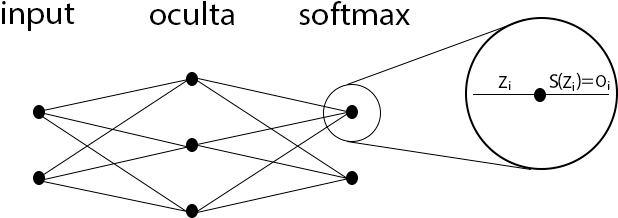
\includegraphics[scale=0.4]{imagenes/NN_softmax.jpg}  
	\caption{Estructura de una red totalmente conectada con una capa oculta, y con softmax en la última capa}
	\label{fig:nn_softmax_1_capa}
\end{figure}

Según esta notación, la función de error \ref{fig:loss_func_softmax} se convierte en la fórmula \ref{cross_entropy_notacion}.

\begin{gather}
	E = - \sum_{i=1}^{N}  [y_i * ln(O_i)] 
	\label{cross_entropy_notacion}
\end{gather}

De este modo, se define el cálculo del gradiente de la pérdida, con respecto a cada neurona de entrada $Z_k$, de la capa SoftMax, según la fórmula \ref{gradiente_softmax} \cite{Cross_entropy_backprop} \cite{Cross_entropy_backprop_grad_input}. Para obtener una explicación detallada, y un desarrollo completo sobre los orígenes de dicha fórmula, consulte el apéndice \ref{softmax_apendice}.

\begin{gather}
	\frac{\partial E}{\partial Z_k} = O_k - y_k = gradiente\_Z_k
	\label{gradiente_softmax}
\end{gather}


\section{Retropropagación en redes neuronales rotalmente conectadas}

En esta sección, se analizará el cálculo del gradiente de la pérdida con respecto a cada parámetro entrenable de una red neuronal totalmente conectada, así como con respecto a la entrada y a la salida de cada capa. De este modo, se presentarán los cálculos aplicables a cualquier tipo de red totalmente conectada. Para obtener una explicación detallada, y un desarrollo completo sobre los orígenes de cada fórmula planteada en esta sección, se recomienda encarecidamente consultar el apéndice \ref{backprop_fully_apendice}.\\

Tal y como se muestra en la Figura \ref{fig:nn_softmax_1_capa}, se definen como capas ocultas todas aquellas capas situadas entre la capa de entrada y la capa de salida.
En particular, se definen como capas ocultas ``intermedias'' todas las capas, exceptuando la última de ellas, dado que estas capas comparten la mayoría de los cálculos asociados a la retropropagación. En consecuencia, una red neuronal totalmente conectada puede dividirse en 4 grupos $\{$capa de entrada, capas ocultas intermedias, última capa oculta, capa de salida o capa softmax$\}$. \\
A continuación, se realiza el cálculo necesario para la retropropagación de una capa de neuronas \textit{l} específica. Suponemos que la capa \textit{l+1} tiene \textit{Q} neuronas, la capa \textit{l-1} tiene \textit{K} neuronas, y que todas las capas ocultas intermedias usan ReLU como función de activación. \\

\subsection{Gradiente respecto a la entrada de la capa}

\begin{figure}[H]
	\centering
	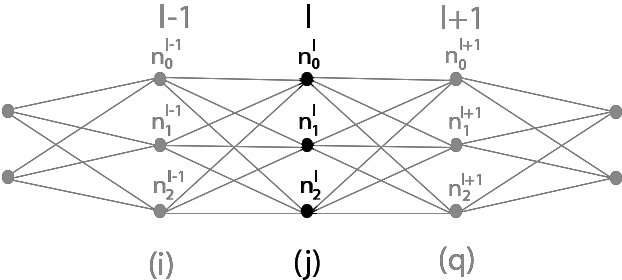
\includegraphics[scale=0.35]{imagenes/conclusion_capa_l.jpg}  
	\caption{Retropropagación en la capa l}
	\label{fig:conclusion_capa_l}
\end{figure}

La Figura \ref{fig:conclusion_capa_l} muestra una representación en la que los 'puntos' están interconectados mediante líneas, los cuales representan neuronas artificiales, y los pesos que las conectan, respectivamente. Cada punto corresponde a una neurona, y, cada línea, a un peso. El superíndice indica la capa a la que pertenece una neurona o peso, mientras que el subíndice especifica el número de la neurona o peso en su respectiva capa. En el caso de los pesos, se requieren 2 subíndices para identificar a cada uno, ya que cada peso conecta 2 neuronas. \\
En este contexto, la capa oculta l está compuesta por 3 neuronas, denotadas como $n^{l}_0$, $n^{l}_1$, y $n^{l}_2$. De este modo. se define como $W^{i}_{jq}$ al peso que une las neuronas $n^{i}_j$ y $n^{i+1}_q$. 
Para la neurona $n^l_j$, se denota como $a^l_j$ el valor de la neurona antes de aplicar la función de activación asociada, y como $z^l_j$, el valor obtenido después de aplicar dicha función. 
Además, se define como $gradiente\_a_{{l+1}_q}$ al gradiente de la pérdida con respecto a $a^{l+1}_q$. Asimismo, se denota como $ReLU'(a^l_j)$ a la derivada de la función de activación ReLU aplicada al valor $(a^l_j)$.\\

\begin{gather}
	\frac{\partial E_{total}}{\partial a^l_j} = \sum_{q=1}^Q  gradiente\_a_{{l+1}_q} * W^l_{ij} * ReLU'(a^l_j) \label{grad_input_l_4}
\end{gather}

La fórmula \ref{grad_input_l_4}, ilustra el cálculo necesario para determinar el gradiente de la función de pérdida, con respecto a la neurona de entrada j, de una capa oculta intermedia \textit{l}, $\frac{\partial E_{total}}{\partial a^l_j}$, a partir del gradiente de la función de pérdida, con respecto a la entrada de capa \textit{l+1}, $gradiente\_a_{{l+1}_q}$.


\subsection{Gradiente respecto a los pesos}

\begin{figure}[H]
	\centering
	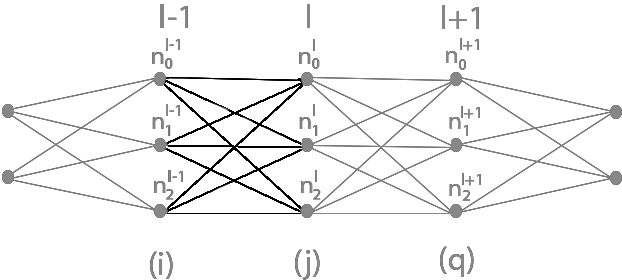
\includegraphics[scale=0.35]{imagenes/conclusion_pesos.jpg}  
	\caption{Retropropagación respecto a los pesos entre la capa l-1 y l}
	\label{fig:conclusion_pesos}
\end{figure}

\begin{gather}
	\frac{\partial E_{total} }{\partial W^{l-1}_{ij} } = gradiente\_h_{l_j} * z^{l-1}_i \label{grad_w_l_3}
\end{gather}

La fórmula \ref{grad_w_l_3}, detalla el cálculo necesario para determinar el gradiente de la pérdida, con respecto a los pesos entre las capas ocultas \textit{l} y \textit{l-1}.

\subsection{Gradiente respecto a sesgos}

\begin{gather}
	\frac{\partial E}{\partial b^l_j} = gradiente\_h_{l_j} \label{grad_b_l_3}
\end{gather}

La fórmula \ref{grad_b_l_3} muestra el cálculo necesario para determinar el gradiente de la función de pérdida con respecto a los sesgos de la capa oculta \textit{l}.

\section{Paralelización mediante OpenMP}

\subsubsection{Tipos de paralelismo}

El entrenamiento de una red neuronal convolucional (CNN) se puede paralelizar de diversas maneras. Cuando el modelo se divide entre varios ordenadores que son entrenados con los mismos datos, se conoce \textbf{paralelismo del modelo} \cite{data_model_parallelism} (por ejemplo, asignando una capa por computador). Por otro lado, cuando se distribuyen los datos entre múltiples nodos, pero se utiliza el mismo modelo para el entrenamiento en cada uno de ellos, se denomina \textbf{paralelismo de datos} \cite{model_parallelism}. En este proyecto, la implementación con OpenMP se basará en un paralelismo de datos, mientras que las implementaciones heterogéneas, utilizando CUDA y cuDNN, se fundamentarán en el paralelismo del modelo. \\

\subsubsection{Paralelismo en SGD con OpenMP}
\begin{algorithm}[H]
	\caption{Descenso del gradiente estocástico} 
	\begin{algorithmic}
		\State Datos de entrenamiento $D=\{(x_1, y_1), (x_2, y_2), ..., (x_N, y_N)\}$.
		
		\For{cada trabajador $t =0, ..., T-1$ en paralelo}
		\For{época $p\in\{0, ..., P-1\}$}
			\State Desordenar vector de datos D.
				\For{cada mini batch $m =0, ..., M-1$}
					\State Inicializar $gradientes^t$ a 0.
					\State Reparto de datos del batch m al trabajador t
					\State Realizar propagación hacia delante
					\State Obtener error total con la función de pérdida
					\State Cada trabajador t realiza la propagación hacia 
					\State detrás y obtiene el gradiente con respecto a 
					\State cada parámetro del modelo.
					
					\State Acumular gradientes obtenidos por cada trabajador t.
					\State Actualizar parámetros.
					
				\EndFor
			\EndFor
		\EndFor
	\end{algorithmic}
\end{algorithm}

La naturaleza iterativa del algoritmo del descenso del gradiente estocástico, podría parecer un impedimento para la paralelización del entrenamiento del modelo, ya que, la iteración \textit{i}, depende del resultado obtenido en la iteración \textit{i-1}. Sin embargo, tal y como se expone en \cite{CNN_parallel_Stanford}, \cite{CNN_parallel_International_Conference}, y \cite{CNN_parallel_Ome_Weird_Trick}, es posible implementar paralelismo en cada iteración del proceso. \\
En cada época el modelo, se entrena con \textit{M} subconjuntos de $N_m$ datos, los cuales son disjuntos entre sí. Dados \textit{T} ``trabajadores'' o procesos paralelos, cada subconjunto de $N_m$ datos (mini-batch), puede dividirse en \textit{T} subconjuntos de $\frac{N_m}{T}$ datos, asignando cada uno a un trabajador diferente.\\
De acuerdo con este enfoque, los datos de entrenamiento se distribuyen entre los distintos trabajadores \textit{T} tanto para la propagación hacia delante como para la retropropagación posterior. En el caso de la retropropagación, se debe acumular el gradiente de la pérdida con respecto a cada parámetro obtenido por cada trabajor. Una vez en posesión este gradiente `total', se procede a la actualización de los parámetros del modelo.

\section{Retropropagación en capas convolucionales}

\begin{figure}[H]
	\centering
	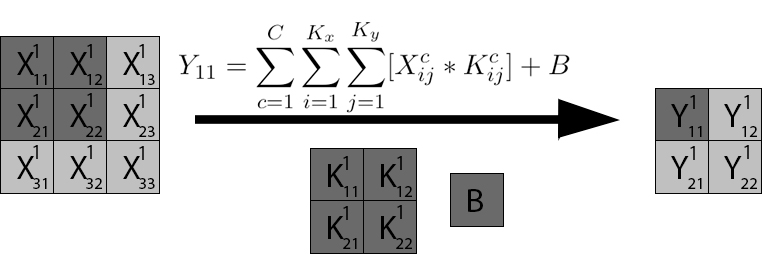
\includegraphics[width=0.8\linewidth]{imagenes/conv_ejemplo_backprop_1.jpg} 
	\caption{Ejemplo de propagación hacia delante en una capa convolucional}
	\label{fig:ejemplo_forward_prop_convolucional}
\end{figure}

La figura \ref{fig:ejemplo_forward_prop_convolucional} ilustra el cálculo de $Y^1_{11}$ para un ejemplo de propagación hacia delante concreto. En dicha figura, \textit{C} representa el número de canales de profundidad del volumen de entrada \textit{X}, mientras que ${K_x}$ y ${K_y}$ se refieren al número de filas y columnas del kernel \textit{K} utilizado, respectivamente. \\
Siguiendo la notación empleada en secciones anteriores, se denotará por $A^c_{ij}$ al valor de $X^c_{ij}$ antes de aplicar la función de activación correspondiente, y por $Z^c_{ij}$ al valor resultante después de aplicar dicha función. Para obtener más detalles, se recomienda consultar el apéndice \ref{backprop_conv_apendice}.

\subsubsection{Sumatoria de gradientes}

\begin{gather}
	\frac{\partial E}{\partial K^c_{11}} = \sum_{i=1}^{I}\sum_{j=1}^{J}  [\frac{\partial E}{\partial Y^c_{ij}} * \frac{\partial Y^c_{ij}}{\partial K^c_{11}}] \notag \\
	\frac{\partial E}{\partial X^c_{11}} = \sum_{i=1}^{I}\sum_{j=1}^{J}  [\frac{\partial E}{\partial Y^c_{ij}} * \frac{\partial Y^c_{ij}}{\partial Z^c_{11}} * \frac{\partial Z^c_{ij}}{\partial A^c_{11}}] \notag 
\end{gather}

Para calcular el gradiente de la función de error con respecto a cada peso ${K_{xy}}$ o entrada ${X_{xy}}$, se debe realizar una sumatoria del gradiente correspondiente sobre cada valor de salida producido por la convolución. En el caso de los pesos asociados a un canal de profundidad $c \in C$, cada peso ${K_{xy}}$ se empleó en el cálculo de cada valor $Y^c_{ij}$. Por otro lado, los valores de la entrada ${X_{xy}}$ contribuyen al cálculo de varios valores de salida $\{Y_1, Y_2\} \in Y$. Este proceso fue detallado anteriormente en la sección \ref{intro_CNN}, y se aborda con mayor profundidad en el apéndice \ref{backprop_conv_apendice}.

\subsubsection{Gradiente de $Y^c_{11}$}

\begin{gather}
	Y^c_{11} = Z^c_{11} * K^c_{11} + Z^c_{12} * K^c_{12} + Z^c_{21} * K^c_{21} + Z^c_{22} * K^c_{22} \label{grad_y11_k_11} \\
	\frac{\partial Y^c_{11}}{\partial K^c_{xy}} = \frac{\partial (Z^c_{11} * K^c_{11} + Z^c_{12} * K^c_{12} + Z^c_{21} * K^c_{21} + Z^c_{22} * K^c_{22})}{\partial K^c_{xy}} \label{grad_y11_k_12} \\
	\frac{\partial Y^c_{11}}{\partial K^c_{11}} = Z^c_{11}, \hspace{10mm} \frac{\partial Y^c_{11}}{\partial K^c_{12}} = Z^c_{12} \label{grad_y11_k_21}\\
	\frac{\partial Y^c_{11}}{\partial K^c_{21}} = Z^c_{21}, \hspace{10mm} \frac{\partial Y^c_{11}}{\partial K^c_{22}} = Z^c_{22} \label{grad_y11_k_22}
\end{gather}

\begin{gather}
	\frac{\partial Y^c_{11}}{\partial Z^c_{11}} = K^c_{11}, \hspace{10mm} \frac{\partial Y^c_{11}}{\partial Z^c_{12}} = K^c_{12}, \hspace{10mm} \frac{\partial Y^c_{11}}{\partial Z^c_{13}} = 0 \label{grad_y11_z_1} \\
	\frac{\partial Y^c_{11}}{\partial Z^c_{21}} = K^c_{21}, \hspace{10mm} \frac{\partial Y^c_{11}}{\partial Z^c_{22}} = K^c_{22}, \hspace{10mm} \frac{\partial Y^c_{11}}{\partial Z^c_{23}} = 0 \label{grad_y11_z_2} \\
	\frac{\partial Y^c_{11}}{\partial Z^c_{31}} = 0, \hspace{15mm} \frac{\partial Y^c_{11}}{\partial Z^c_{32}} = 0, \hspace{15mm} \frac{\partial Y^c_{11}}{\partial Z^c_{33}} = 0 \label{grad_y11_z_3}
\end{gather}

La fórmula \ref{grad_y11_k_11}, presenta una descomposición de $Y^c_{11}$ en términos de $Z$ y $K$. Esto, es esencial para el cálculo del gradiente, tanto con respecto a Z, (como se detalla en las fórmulas \ref{grad_y11_z_1}, \ref{grad_y11_z_2}, \ref{grad_y11_z_3}), como con respecto a K, (como se muestra en las fórmulas \ref{grad_y11_k_12}, \ref{grad_y11_k_21}, \ref{grad_y11_k_22}). Esta descomposición, permite calcular el gradiente de $Y^c_{11}$ con respecto a cada parámetro de la capa convolucional. \\
Cabe destacar que, para calcular el gradiente con respecto a cada valor del volumen de entrada (X), también debe calcularse la derivada de la función de activación asociada a dicha capa. Es decir, $\frac{\partial Z}{\partial A}$. Sin embargo, dado que este proceso ha sido abordado en secciones anteriores, se omitirá en esta ocasión, al igual que el cálculo del gradiente con respecto al sesgo de cada capa. El propósito de esta omisión es evitar cálculos redundantes y concentrar la atención en los aspectos más relevantes e innovadores. No obstante, es importante señalar que todos los cálculos discutidos en esta documentación, y más, están implementados en el código correspondiente, lo que garantiza que este conocimiento se ha aplicado y verificado en la práctica. \\
Además, dado que todo ha sido realizado manualmente por la misma persona, la mayoría de las variables e índices utilizados en la documentación coinciden perfectamente o son muy similares a los empleados en el código. Esto asegura que cualquier lector con conocimientos básicos de programación pueda comprender gran parte de las implementaciones desarrolladas en este proyecto.

\subsubsection{Gradiente con respecto a los pesos como convolución}

Finalmente, se procede al cálculo de la suma total de gradientes con respecto a cada peso de la capa, conforme a las fórmulas \ref{grad_Y_K_1}, \ref{grad_Y_K_2}, \ref{grad_Y_K_3}, y \ref{grad_Y_K_4}. Para una explicación detallada del cálculo y los fundamentos de cada fórmula, se recomienda consultar el apéndice \ref{backprop_conv_apendice}. Los gradientes resultantes, revelan un patrón claro que refleja la contribución de cada peso en el cálculo del error total.

\begin{gather}
	\frac{\partial E}{\partial K^c_{11}} = \frac{\partial E}{\partial Y^c_{11}} * Z^c_{11} + \frac{\partial E}{\partial Y^c_{12}} * Z^c_{12} + \frac{\partial E}{\partial Y^c_{21}} * Z^c_{21} + \frac{\partial E}{\partial Y^c_{22}} * Z^c_{22} \label{grad_Y_K_1} \\
	\frac{\partial E}{\partial K^c_{12}} = \frac{\partial E}{\partial Y^c_{11}} * Z^c_{12} + \frac{\partial E}{\partial Y^c_{12}} * Z^c_{13} + \frac{\partial E}{\partial Y^c_{21}} * Z^c_{22} + \frac{\partial E}{\partial Y^c_{22}} * Z^c_{23} \label{grad_Y_K_2} \\	
	\frac{\partial E}{\partial K^c_{21}} = \frac{\partial E}{\partial Y^c_{11}} * Z^c_{21} + \frac{\partial E}{\partial Y^c_{12}} * Z^c_{22} + \frac{\partial E}{\partial Y^c_{31}} * Z^c_{21} + \frac{\partial E}{\partial Y^c_{22}} * Z^c_{32} \label{grad_Y_K_3} \\
	\frac{\partial E}{\partial K^c_{22}} = \frac{\partial E}{\partial Y^c_{11}} * Z^c_{22} + \frac{\partial E}{\partial Y^c_{12}} * Z^c_{23} + \frac{\partial E}{\partial Y^c_{31}} * Z^c_{32} + \frac{\partial E}{\partial Y^c_{22}} * Z^c_{33} \label{grad_Y_K_4}
\end{gather}

Como se observa en los cálculos realizados, estos coinciden con una operación de convolución entre la entrada \textit{X} y el gradiente respecto a la capa de salida \textit{Y}. Este procedimiento se detalla en la Figura \ref{fig:conv_backprop_como_convolucion_X_Y} \cite{conv_backprop}.

\begin{figure}[H]
	\centering
	\begin{subfigure}{.5\textwidth}
		\hspace{-25mm}
		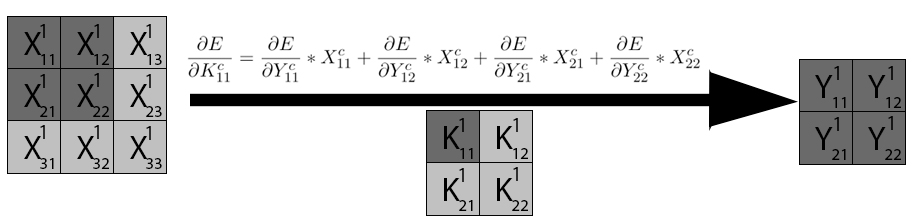
\includegraphics[width=1.4\linewidth]{imagenes/conv_backprop_1.jpg}  
		\caption{Cálculo de $\frac{\partial E}{\partial K^1_{11}}$}
	\end{subfigure}%
	\begin{subfigure}{.5\textwidth}
		\hspace{5mm}
		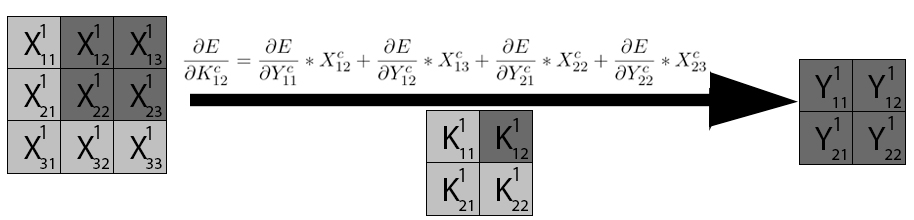
\includegraphics[width=1.4\linewidth]{imagenes/conv_backprop_2.jpg}  
		\caption{Cálculo de $\frac{\partial E}{\partial K^1_{12}}$}
	\end{subfigure}
	\vspace{5mm}
	\begin{subfigure}{.5\textwidth}
		\hspace{-25mm}
		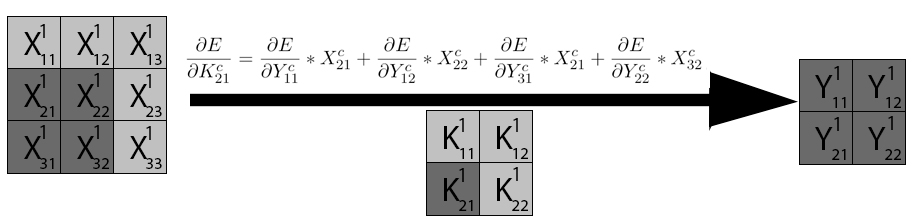
\includegraphics[width=1.4\linewidth]{imagenes/conv_backprop_3.jpg}  
		\caption{Cálculo de $\frac{\partial E}{\partial K^1_{21}}$}
	\end{subfigure}%
	\begin{subfigure}{.5\textwidth}
		\hspace{5mm}
		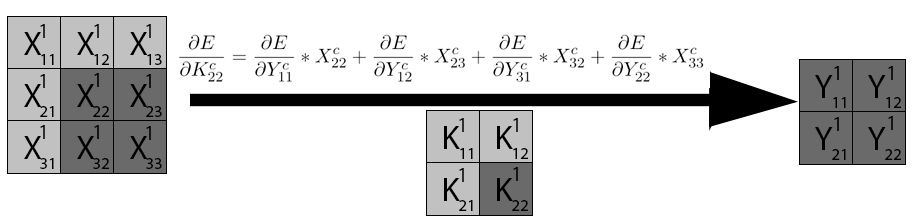
\includegraphics[width=1.4\linewidth]{imagenes/conv_backprop_4.jpg}  
		\caption{Cálculo de $\frac{\partial E}{\partial K^1_{22}}$}
	\end{subfigure}
	\caption{Cálculo del gradiente de la pérdida con respecto a cada filtro como convolución entre la entrada X y la salida Y}
	\label{fig:conv_backprop_como_convolucion_X_Y}
\end{figure}

En la figura \ref{fig:conv_backprop_como_convolucion_X_Y}, cada subfigura $\{(a), (b), (c), (d)\}$ representa el cálculo del gradiente con respecto a un peso específico. Aunque la representación puede parecer algo diferente a simple vista, los cálculos son esencialmente los mismos que los obtenidos anteriormente, con la única diferencia en la forma en que se visualizan.

\subsubsection{Gradiente con respecto a la entrada como convolución}

Por razones de simplicidad, y en consonancia con las recomendaciones de expertos, y la experiencia personal, se empleará ReLU como función de activación en las capas convolucionales. Dado que, la derivada de esta función ya ha sido previamente calculada, (véase la fórmula \ref{deriv_relu}), se considerará esta información para los cálculos subsiguientes.


\begin{gather}
	\frac{\partial E}{\partial A^c_{11}} = \frac{\partial E}{\partial Y^c_{11}} * K^c_{11} *  ReLU'(A^c_{11}) \notag \\
	\frac{\partial E}{\partial A^c_{12}} = (\frac{\partial E}{\partial Y^c_{11}} * K^c_{12} + \frac{\partial E}{\partial Y^c_{12}} * K^c_{11}) * ReLU'(A^c_{12}) \notag \\
	\frac{\partial E}{\partial A^c_{13}} = \frac{\partial E}{\partial Y^c_{12}} * K^c_{12} * ReLU'(A^c_{13}) \notag \\
	\frac{\partial E}{\partial A^c_{21}} = (\frac{\partial E}{\partial Y^c_{11}} * K^c_{21} + \frac{\partial E}{\partial Y^c_{21}} * K^c_{11}) * ReLU'(A^c_{21}) \notag \\
	\frac{\partial E}{\partial A^c_{22}} = (\frac{\partial E}{\partial Y^c_{11}} * K^c_{22} + \frac{\partial E}{\partial Y^c_{12}} * K^c_{21} + \frac{\partial E}{\partial Y^c_{21}} * K^c_{12} + \frac{\partial E}{\partial Y^c_{22}} * K^c_{11}) * ReLU'(A^c_{22}) \notag \\
	\frac{\partial E}{\partial A^c_{23}} = (\frac{\partial E}{\partial Y^c_{12}} * K^c_{22} + \frac{\partial E}{\partial Y^c_{22}} * K^c_{12}) * ReLU'(A^c_{22})\notag \\
	\frac{\partial E}{\partial A^c_{31}} = \frac{\partial E}{\partial Y^c_{21}} * K^c_{21} * ReLU'(A^c_{31})\notag \\
	\frac{\partial E}{\partial A^c_{32}} = (\frac{\partial E}{\partial Y^c_{21}} * K^c_{22} + \frac{\partial E}{\partial Y^c_{22}} * K^c_{21}) * ReLU'(A^c_{32}) \notag \\
	\frac{\partial E}{\partial A^c_{33}} = \frac{\partial E}{\partial Y^c_{22}} * K^c_{22} * ReLU'(A^c_{33}) \notag
\end{gather}

Tal y como se observa en los cálculos obtenidos, estos corresponden a una convolución completa entre el gradiente con respecto a la capa de salida (Y) y los pesos (K), invertidos tanto horizontal como verticalmente. El proceso de cálculo del gradiente con respecto a cada valor de entrada $x \in X$ se presenta en detalle en la figura \ref{fig:conv_backprop_como_convolucion_Y_W}, mientras que la manera de invertir los pesos se ilustra en la figura \ref{fig:flip_W} \cite{conv_backprop}.

\begin{figure}[H]
	\centering
	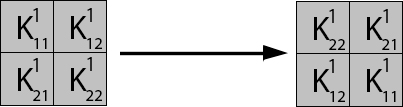
\includegraphics[width=0.8\linewidth]{imagenes/flip_pesos.jpg}  
	\caption{Inversión de los pesos en K tanto horizontal como verticalmente}
	\label{fig:flip_W}
\end{figure}

\begin{figure}[H]
	\centering
	\begin{subfigure}{.5\textwidth}
		\hspace{-25mm}
		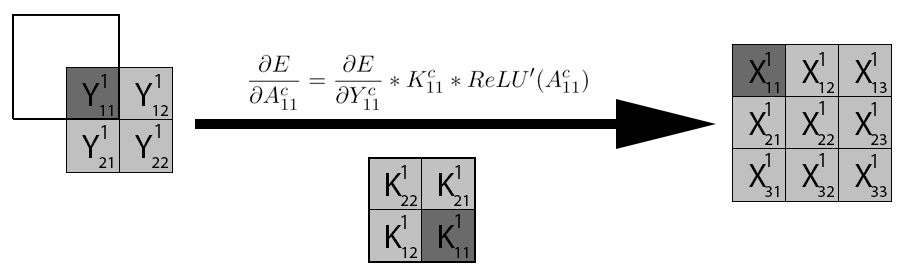
\includegraphics[width=1.4\linewidth]{imagenes/conv_back_entrada_1.jpg}  
		\caption{Gradiente con respecto a $X^1_{11}$}
	\end{subfigure}%
	\begin{subfigure}{.5\textwidth}
		\hspace{5mm}
		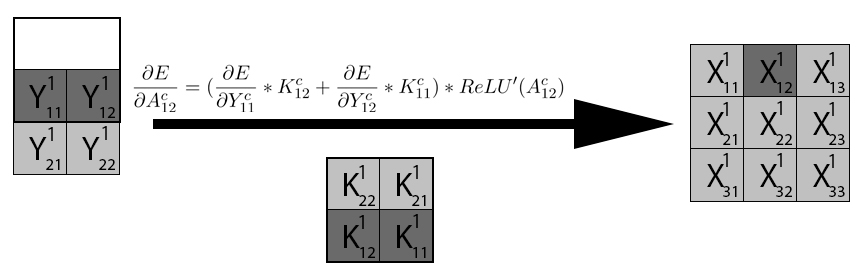
\includegraphics[width=1.4\linewidth]{imagenes/conv_back_entrada_2.jpg}  
		\caption{Gradiente con respecto a $X^1_{12}$}
	\end{subfigure}
	\vspace{5mm}
	\begin{subfigure}{.5\textwidth}
		\hspace{-25mm}
		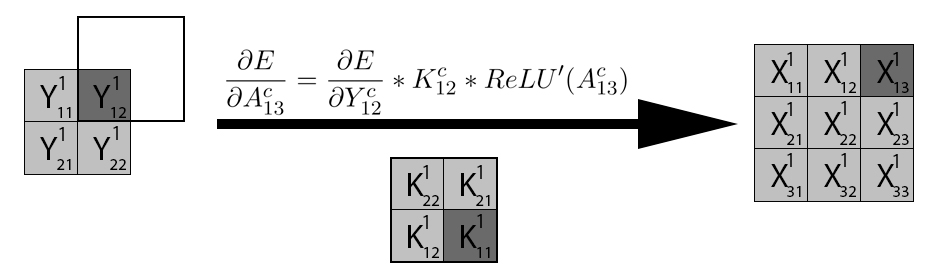
\includegraphics[width=1.4\linewidth]{imagenes/conv_back_entrada_3.jpg}  
		\caption{Gradiente con respecto a $X^1_{13}$}
	\end{subfigure}%
	\begin{subfigure}{.5\textwidth}
		\hspace{5mm}
		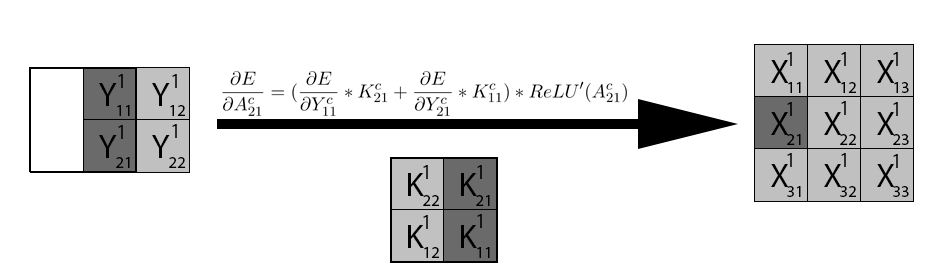
\includegraphics[width=1.4\linewidth]{imagenes/conv_back_entrada_4.jpg}  
		\caption{Gradiente con respecto a $X^1_{21}$}
	\end{subfigure}
	\vspace{5mm}
	\begin{subfigure}{.5\textwidth}
		\hspace{-25mm}
		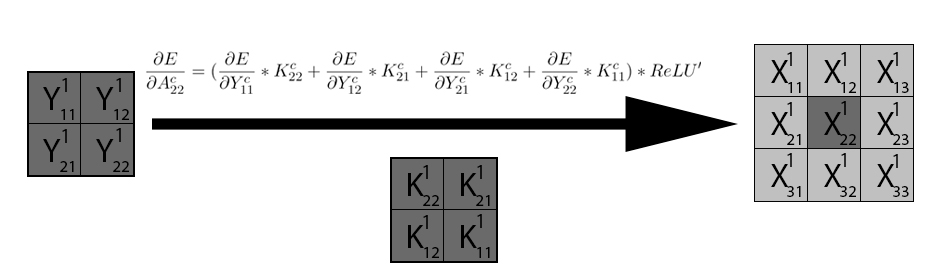
\includegraphics[width=1.4\linewidth]{imagenes/conv_back_entrada_5.jpg}  
		\caption{Gradiente con respecto a $X^1_{22}$}
	\end{subfigure}%
	\begin{subfigure}{.5\textwidth}
		\hspace{5mm}
		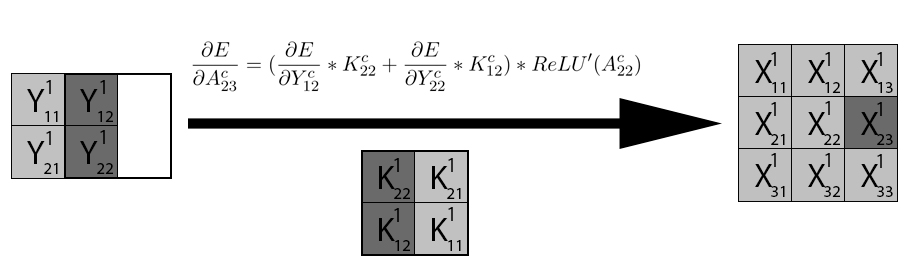
\includegraphics[width=1.4\linewidth]{imagenes/conv_back_entrada_6.jpg}  
		\caption{Gradiente con respecto a $X^1_{23}$}
	\end{subfigure}
	\vspace{5mm}
	\begin{subfigure}{.5\textwidth}
		\hspace{-25mm}
		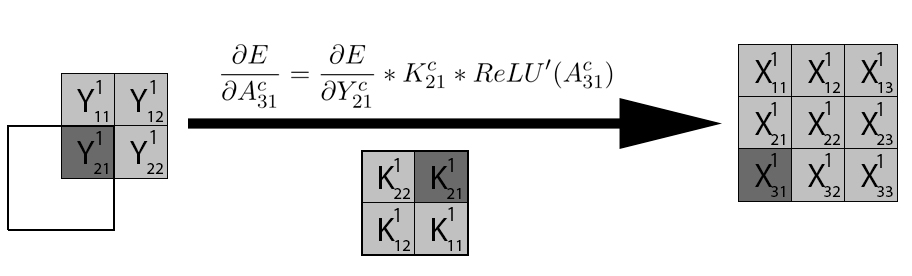
\includegraphics[width=1.4\linewidth]{imagenes/conv_back_entrada_7.jpg}  
		\caption{Gradiente con respecto a $X^1_{31}$}
	\end{subfigure}%
	\begin{subfigure}{.5\textwidth}
		\hspace{5mm}
		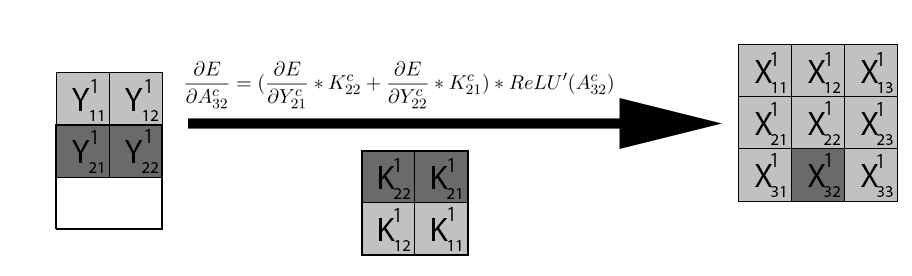
\includegraphics[width=1.4\linewidth]{imagenes/conv_back_entrada_8.jpg}  
		\caption{Gradiente con respecto a $X^1_{32}$}
	\end{subfigure}
	\vspace{5mm}
	\begin{subfigure}{.5\textwidth}
		\hspace{-25mm}
		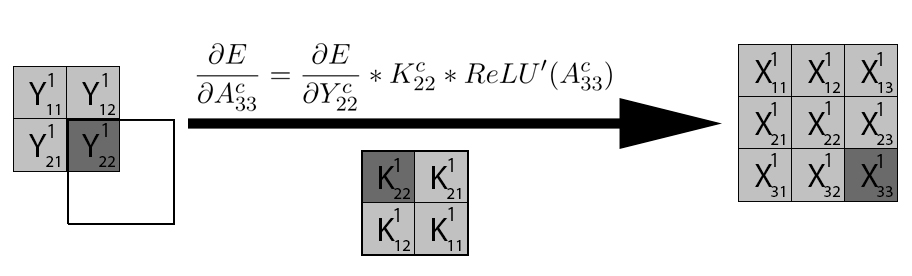
\includegraphics[width=1.4\linewidth]{imagenes/conv_back_entrada_9.jpg}  
		\caption{Gradiente con respecto a $X^1_{33}$}
	\end{subfigure}
	\caption{Cálculo del gradiente de la pérdida con respecto a cada valor de entrada como convolución entre los pesos K y la salida Y}
	\label{fig:conv_backprop_como_convolucion_Y_W}
\end{figure}

Una vez más, los cálculos presentados en la Figura \ref{fig:conv_backprop_como_convolucion_Y_W} coinciden perfectamente con los obtenidos anteriormente, ya que son idénticos. La única diferencia radica en la manera de presentación, la cual ha sido adaptada para ofrecer una mejor comprensión y generalización del proceso. Esta adaptación facilita la automatización de los cálculos y permite una implementación más eficiente en el código.


\subsection{Retropropagación en capas convolucionales con relleno}

Para realizar la retropropagación en una capa convolucional sin relleno, con respecto a la entrada, se emplea una convolución completa. En contraste, para la retropropagación en una capa convolucional con relleno, con respecto a la entrada, se utiliza una convolución sin relleno. Ambos tipos de convoluciones, así como el cálculo detallado de la retropropagación en cada caso, se examinan exhaustivamente en el apéndice \ref{backprop_conv_apendice}.

\begin{figure}[H]
	\centering
	\begin{subfigure}{.5\textwidth}
		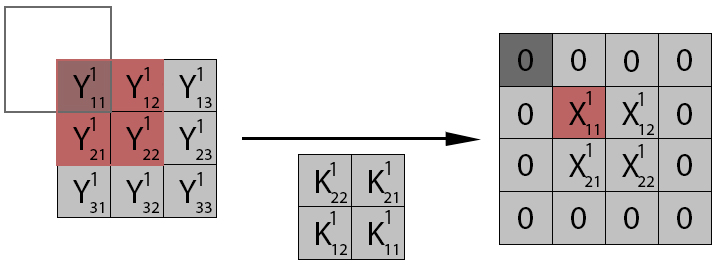
\includegraphics[width=1.4\linewidth]{imagenes/full_vs_normal_conv_1.jpg}  
		\caption{Retropropagación con un nivel de relleno}
	\end{subfigure}
	
	\vspace{5mm}
	\begin{subfigure}{.5\textwidth}
		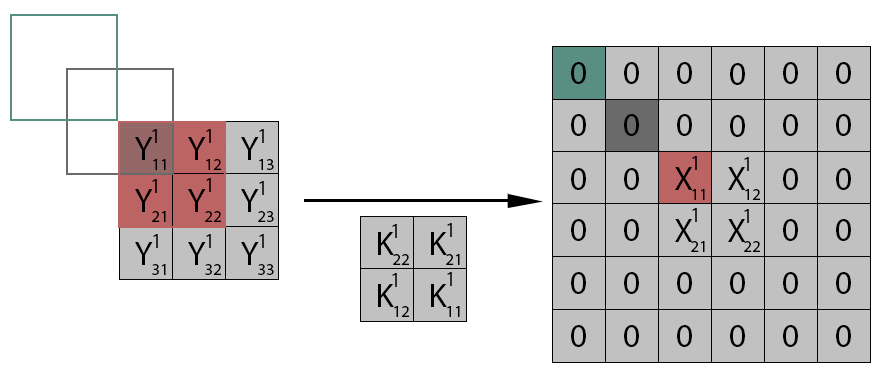
\includegraphics[width=1.4\linewidth]{imagenes/full_vs_normal_conv_2.jpg}  
		\caption{Retropropagación con dos niveles de relleno}
	\end{subfigure}
	\caption{Cálculo del gradiente de la pérdida con respecto a la entrada X con uno y dos niveles de relleno}
	\label{fig:conv_full_vs_normal}
\end{figure}

La razón detrás de esta diferencia se detalla en la figura \ref{fig:conv_full_vs_normal}. En el caso de una convolución con relleno completo, los gradientes se calculan comenzando desde la esquina superior izquierda de la entrada X. Sin embargo, dado que dicha entrada X incluye relleno, no es necesario calcular los gradientes en las posiciones de relleno, ya que estos valores no influyen en los cálculos posteriores.
